\documentclass[]{../util/ColumbiaAssm}
\usepackage{../util/W4400Student}


%%%% FOR EXAM PACKAGE
\printanswers % If you don't want to print answers
\addpoints % if you want to count the points
% \noaddpoints % if you don't want to count the points
% Specifies the way question are displayed:
%\qformat{\textbf{Question \thequestion}\quad(\thepoints)\hfill}
%\qformat{Question \thequestion:\hfill }
\qformat{\thequestion. \textbf{\thequestiontitle} (\thepoints)\hfill }
\usepackage{color} % defines a new color
\definecolor{SolutionColor}{rgb}{0.1,0.1,0.1} % light blue
%\shadedsolutions % defines the style of the solution environment
\framedsolutions % defines the style of the solution environment
% Defines the title of the solution environment:
\renewcommand{\solutiontitle}{\noindent\emph{Solution:~~~}\noindent}


\usepackage{latexsym}
\usepackage{amsmath,amsfonts,amssymb}
\usepackage{epic}
\usepackage{eepic}
\usepackage{epsfig}

\begin{document}
  \makeAssmHeader{1}{Due: Tuesday 09 February 2016}
  \vspace{-2cm}


\AddSubmissionRules

  \def\mean#1{\mbox{E}\left[ #1 \right]}
\def\var#1{\mbox{Var}\left[ #1 \right]}
\def\cov#1{\mbox{Cov}\left[ #1 \right]}
\def\cmean[#1]#2{\mbox{E}_{#1}\left[ #2 \right]}
\def\skew#1{\mbox{Skew}\left[ #1 \right]}
\def\kurt#1{\mbox{Kurt}\left[ #1 \right]}
\def\Prob#1{\mbox{Pr}\lbrace #1 \rbrace}
\def\cProb[#1]#2{\mbox{Pr}_{#1}\lbrace #2\rbrace}
\def\Pmass#1{P\left( #1 \right)}
\def\Pdens#1{p\left( #1 \right)}
\def\iid{i.~i.~d.\ }
\def\Iid{I.~i.~d.\ }
\def\argmax#1{\textrm{arg}\max_{#1}}
\def\argmin#1{\textrm{arg}\min_{#1}}
\def\kld#1{D_{\mbox{\tiny KL}}\left( #1 \right)}
\def\hist{\mathbf{h}}
\def\entropy#1{H\lbrack #1 \rbrack}
\def\nBins{N_{\mbox{\tiny bins}}}
\newcommand{\bs}[1]{\boldsymbol{#1}}


  \vspace{0.5cm}

  \def\Rd{\mathbb{R}^d}
  \def\indH{\mbox{\tiny H}}
  \def\v{\mathbf{v}}
  \def\sign{\mbox{sgn}}
  \def\sp#1{\left< #1\right>}
  \def\train{\tilde{\x}}
  \def\trainlabel{\tilde{y}}
  \def\x{\mathbf{x}}
  \def\y{\mathbf{y}}
  \def\z{\mathbf{z}}


\begin{questions}

%%%%%%%%%%%%%%%%%%%%%%%%%%%%
\titledquestion{Naive Bayes}[20]

    Consider a classification problem with training data $\lbrace
    (\train_1,\trainlabel_1),\ldots,(\train_n,\trainlabel_n)\rbrace$
    and three classes $\mathcal{C}_1$, $\mathcal{C}_2$ and
    $\mathcal{C}_3$. The sample space is $\mathbb{R}^5$, so each
    data point is of the form $\x=(x^{(1)},\ldots,x^{(5)})$.
    Suppose we have reason to believe that the
    distribution of each
    class is reasonably well-approximated by a spherical
    (unit-variance) Gaussian, i.e.\ the class-conditional distributions
    are $g(\x|\mu_k,\mathbb{I})$ for class ${k\in\lbrace 1,2,3\rbrace}$.

    \begin{enumerate}
    \item How is the Gaussian assumption translated into a naive Bayes classifier?
      Write out the full formula for the estimated
      class label $\hat{y}_{\mbox{\tiny new}}=f(\x_{\mbox{\tiny new}})$ for a newly observed
      data point $\x_{\mbox{\tiny new}}$.\\
      \textbf{Hint:} This equation should not contain the training
      data, only parameters estimated from the training data.
    \item How do you estimate the parameters of the model? Give the
      estimation equations for (a) the parameters of the
      class-conditional distributions
      and (b) the class prior $P(y=k)$ for each class $\mathcal{C}_k$.
    \item If our assumptions on the data source as described above are accurate,
      do you expect the naive Bayes classifier to perform well? Please explain your answer.
    \end{enumerate}

\begin{solution}
\newline
1a. The Gaussian assumption implies sample independence as there is zero covariance between classes which enables $\Pr(\mathbf{x}|y)$ to be written in the form of a naive Bayes classifier $\prod\limits^{d}_{j=1} \Pr(\mathbf{x}|y)$.\\
1b. $\hat{y}_{new} 
= \underset{y \in \{C_1, C_2, C_3\}}{\arg\max} \Pr(y|\mathbf{x}_{new}) = \underset{y \in \{C_1, C_2, C_3\}}{\arg\max}\Pr(\mathbf{x}_{new}|y)\Pr(y)$, $\Pr(y) = \frac{1}{(2\pi\sigma)^\frac{1}{2}} e^{-\frac{(x-\mu_k)^2}{2}}$\\
2a. For each class $C_k$, $\mu_k = \frac{1}{n_k} \sum\limits_{i=1}^{n_k} \mathbf{x}_k$ \\
2b. $\Pr(y = k) = \frac{\textrm{\# observations in }C_k}{\# \textrm{observations}}$\\
3. Yes. Given that the samples in the training data are parameterised by an identity covariance matrix denoting zero covariance between classes, they fit the sample independence assumption made by the naive Bayes classifier. Hence the classifier would classify the samples well as its assumptions are in line with the nature of the dataset. 
\end{solution}


%%%%%%%%%%%%%%%%%%%%%%%%%%%%
\titledquestion{Maximum Likelihood Estimation}[40]

In this problem, we analytically derive maximum likelihood
estimators for the parameters of an example model
distribution, the gamma distribution.
    
The gamma distribution is univariate (one-dimensional) and
continuous. It is controlled by two parameters, the 
{\em location parameter} $\mu$ and the {\em shape parameter} $\nu$.
%\footnote{In parametric statistics, we usually call parameters
%  shape parameters if they are neither location nor scale parameters.}
For a gamma-distributed random variable $X$, we write
$X\sim\mathcal{G}\left(\mu,\nu\right)$. $\mathcal{G}$ is
defined by the following density function:
\begin{equation}
  \Pdens{ x | \mu,\nu} := \left(\frac{\nu}{\mu}\right)^{\nu}
  \frac{x^{\nu - 1}}{\Gamma\left( \nu \right)}
  \exp\left( -\frac{\nu x}{\mu} \right) \; , \nonumber
\end{equation}
where $x \geq 0$ and $\mu,\nu > 0$.\footnote{ The symbol $\Gamma$ denotes the distribution's
  namesake, the {\em gamma function}, defined by
  \begin{equation*}
    \Gamma\left( \nu \right) := \int_{0}^{\infty} e^{- t} t^{\nu-1}
    dt \; . \nonumber
  \end{equation*} 
  The gamma function is a generalization of the factorial
  to the real line: $\Gamma\left( n \right) = \left(
  n - 1 \right) !$ for all $n\in\mathbf{N}$. Fortunately, we will not
  have to make explicit use of the integral.}
Whenever $\nu > 1$, the gamma density has a single peak, much like
a Gaussian. Unlike the Gaussian, it is not symmetric.
The first two moment statistics of the gamma distribution are
given by
\begin{equation}
  \label{gammaStatistics}
  \mean{X} = \mu \qquad \mbox{ and } \qquad \var{X} = \frac{\mu^2}{\nu}
\end{equation}
for $X\sim\mathcal{G}\left(\mu,\nu\right)$.
The plots in Figure \ref{fig:gamma}
should give you a rough idea of what the
gamma density may look like and how different parameter values
influence its behavior.
\begin{figure}[t]
\begin{center}
  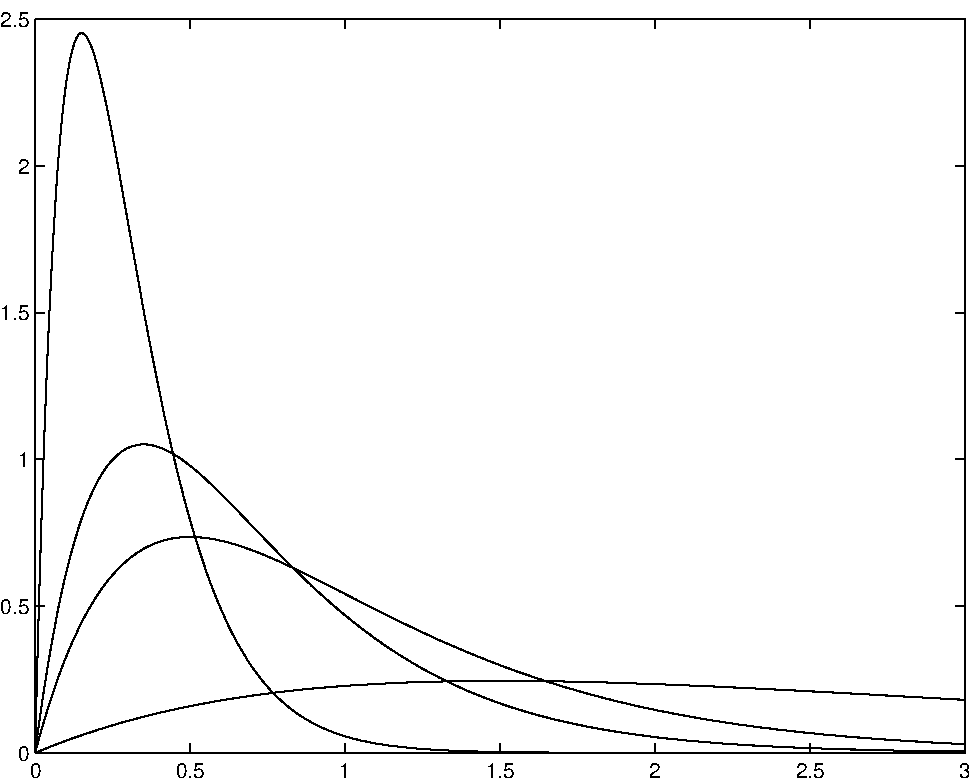
\includegraphics[width=5cm]{analytic_mle__1.pdf}
  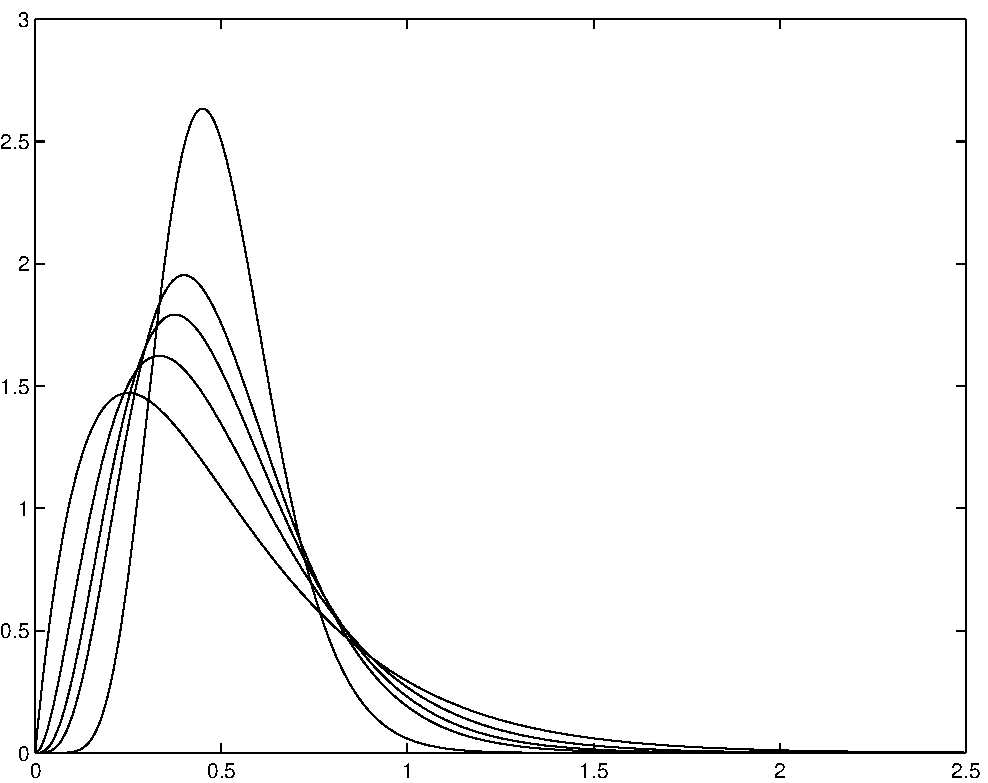
\includegraphics[width=5cm]{analytic_mle__2.pdf}
  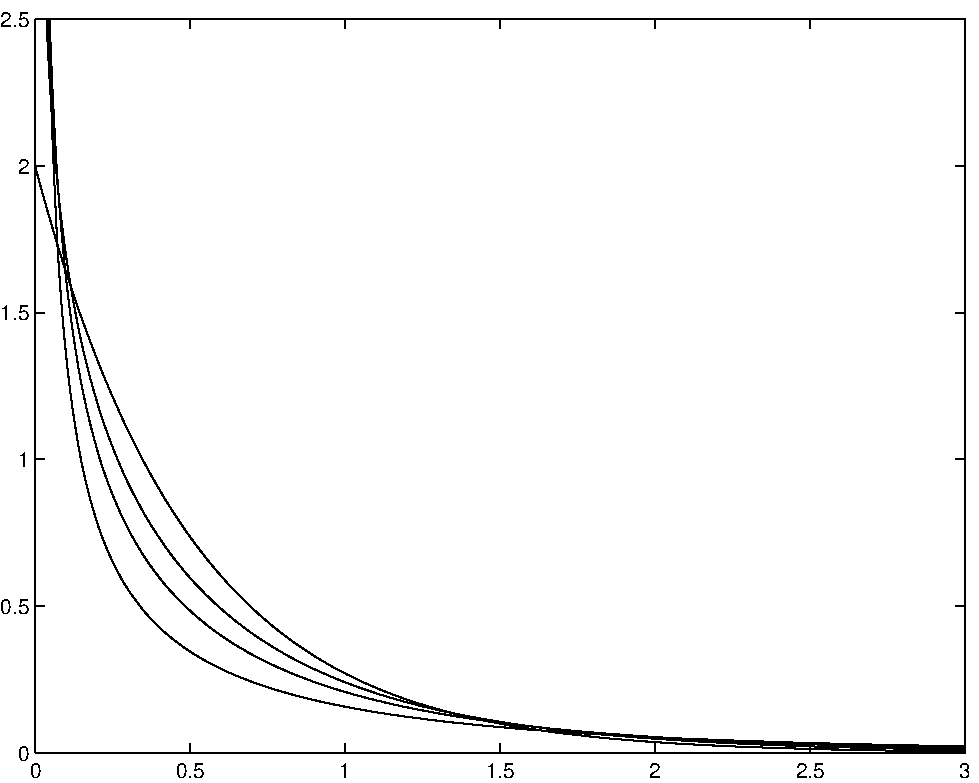
\includegraphics[width=5cm]{analytic_mle__3.pdf}
\end{center}
\caption{
    {\em Left:} The plot shows the density for different values of the
    location parameter ($\mu = 0.3,0.5,1.0,3.0$), with the shape
    parameter fixed to $\nu = 2$.  
    Since $\nu > 1$, the densities peak. As we increase $\mu$, the
    peak moves to the right, and the curve flattens.
    {\em Middle:} For $\mu = 0.5$ fixed, we look at different values of
    the shape parameter ($\nu = 2, 3, 4, 5, 19$). Again, all the
    densities peak, with the peak shifting to the right as we increase $\nu$.
    {\em Right:} If $\nu < 1$, the density turns into a
    monotonously decreasing function. The smaller the value of $\nu$, the
    sharper the curve dips towards the origin. 
}
\label{fig:gamma}
\end{figure}

\newpage
Questions:
    \begin{itemize}
    
    \item (8 points)
      Write the general analytic procedure to obtain the
      maximum likelihood estimator (including logarithmic
      transformation) in the form of a short algorithm or 
      recipe. A few words are enough, but be precise: Write all important
      mathematical operations as formulae. Assume that data is given
      as an \iid sample $x_1,\dots,x_n$. Denote the conditional
      density in question by $\Pdens{x | \theta }$, and the
      likelihood by $l\left( \theta \right)$. Make sure both symbols
      show up somewhere in your list, as well as a logarithm turning 
      a product into a sum.
    \item (16 points)
      Derive the ML estimator for the location parameter
      $\mu$, given data values $x_1,\dots,x_n$. 
      Conventionally, an estimator for a parameter is
      denoted by adding a hat: $\hat{\mu}$.
      Considering the expressions in \eqref{gammaStatistics} for the 
      mean and variance of the gamma distribution, and what you
      know about MLE for Gaussians, the result should not come as a surprise.
    \item (16 points)
      A quick look at the gamma density will tell you that things get
      more complicated for the shape parameter: $\nu$ 
      appears inside the gamma function, and both inside and outside
      the exponential.
      Thus, instead of deriving a formula of the form
      $\hat{\nu}:=\dots$, please show the following:
      Given an \iid data sample $x_1,\dots,x_n$ and the value of
      $\mu$, the ML estimator $\hat{\nu}$ for the gamma distribution shape
      parameter solves the equation
      \begin{equation*}
	\label{nuTranscendentalEquation}
	\sum_{i=1}^{n}\left(
	\ln \left( \frac{x_i \hat{\nu}}{\mu} \right) - \left( \frac{x_i}{\mu} -
	1 \right) - 
	\phi\left( \hat{\nu} \right)
	%	\frac{
	%	  \frac{\partial}{\partial\hat{\nu}}\Gamma\left(\hat{\nu}\right)}{\Gamma\left(
	%	  \hat{\nu} \right)}
	\right) = 0 \; .
      \end{equation*}
      The symbol $\phi$ is a shorthand notation for 
      \begin{equation*}
	\phi\left( \nu \right) := \frac{\frac{\partial\Gamma\left(
	    \nu\right)}{\partial \nu}}{\Gamma\left( \nu \right)} \; .
      \end{equation*}
      In mathematics, $\phi$
      is known as the {\em digamma function}.
    \end{itemize}


\begin{solution}
\newline Part A. \\
1. Set the likelihood function as $L_n (\theta, \mathbf{x}) = \prod\limits^{n}_{i=1} \Pr(x|\theta)$\\
2. Take $\ln$ of $L_n$ to get $\ell_n(\theta, \mathbf{x}) = \ln \prod\limits^{n}_{i=1} \Pr(x|\theta) = \sum\limits^{n}_{i=1} \ln\Pr(x|\theta)$\\
3. Differentiate $\ell_n$ w.r.t. $\theta$ to get $\frac{\partial \ell}{\partial \theta}$ (If $\theta$ is a vector, calculate $\nabla \ell_n$)\\
4. Solve $\frac{\partial \ell}{\partial \theta} = 0$ to get $\hat{\theta}$ (If $\theta$ is a vector, solve $\nabla \ell_n = 0$ to get $\hat{\theta}$)\\ \\
Part B.\\
Get $\frac{\partial \ell}{\partial \mu} = \frac{\partial}{\partial \mu} (n \nu \ln \nu - n \nu \ln \mu + (\nu - 1)\ln(\prod\limits^{n}_{i=1} x) - n\ln(\Gamma(\nu)) - \frac{\nu \sum\limits^{n}_{i=1} x_i}{\mu}) = - \frac{n\nu}{\mu} + \frac{\nu \sum\limits^{n}_{i=1} x_i}{\mu^2}$\\
Equate $- \frac{n\nu}{\mu} + \frac{\nu \sum\limits^{n}_{i=1} x_i}{\mu^2}$ to 0 to get $\frac{n\nu}{\mu} = \frac{\nu \sum\limits^{n}_{i=1} x_i}{\mu^2}$ which provides the estimator for $\mu$, $\hat{\mu} = \frac{1}{n} \sum\limits^{n}_{i=1} x_i$
\newpage
Part C.\\
Get $\frac{\partial \ell}{\partial \mu} = \frac{\partial \ell}{\partial \nu} = n\ln \nu + n - n\ln \mu + \sum\limits^{n}_{i=1} \ln x - n \frac{\partial}{\partial \nu} \ln(\Gamma(\nu)) - \frac{\sum\limits^{n}_{i=1} x_i}{\mu}$\\
Equate above to 0 and collect terms: 
\begin{itemize}
\item $n\ln \nu - n\ln \mu + \sum\limits^{n}_{i=1} \ln x_i = \sum\limits^{n}_{i=1} \ln \frac{\nu}{\mu} + \sum\limits^{n}_{i=1} \ln x_i = \sum\limits^{n}_{i=1} \ln \frac{x_i \nu}{\mu}$
\item $-\frac{\sum\limits^{n}_{i=1} x_i}{\mu} + n = - \sum\limits^{n}_{i=1} (\frac{x_i}{\mu} - 1)$
\item $- n \frac{\partial}{\partial \nu} \ln(\Gamma(\nu)) = - n \frac{\frac{\partial}{\partial \nu}\Gamma(\nu)}{\Gamma(\nu)} =  - \sum\limits^{n}_{i=1} \frac{\frac{\partial}{\partial \nu}\Gamma(\nu)}{\Gamma(\nu)} = -\sum\limits^{n}_{i=1} \phi(\nu)$
\end{itemize} 
Combine the collected terms to obtain $\sum\limits^{n}_{i=1}(\ln \frac{x_i \nu}{\mu} - (\frac{x_i}{\mu} - 1) - \phi(\nu)) = 0$
%\begin{align*}
%\begin{split}
%
%\end{split}
%\end{align*}


 
\end{solution} 
 
%%%%%%%%%%%%%%%%%%%%%%%%%%%%
\titledquestion{Bayes-Optimal Classifier}[30]

\def\x{\mathbf{x}}
Consider a classification problem with $K$ classes and with observations in
$\mathbb{R}^d$. Now suppose we have access to the true joint density $p(\x,y)$
of the data $\x$ and the labels $y$. From $p(\x,y)$ we can derive the
conditional probability $P(y|\x)$, that is, the posterior probability
of class $y$ given observation $\x$.

In the lecture, we have
introduced a classifier $f_0$ based on $p$, defined as
\begin{equation*}
  f_0(\x):=\argmax{y\in [K]} P(y|\x) \;,
\end{equation*}
the \emph{Bayes-optimal classifier}.

\def\Lzeroone{L^{\mbox{\tiny 0-1}}}

\textbf{Homework question:}
Show that the Bayes-optimal classifier is the classifier which
  minimizes the probability of error, under all classifiers in the
  hypothesis class
  \begin{equation*}
    \mathcal{H}:=\lbrace f\!:\mathbb{R}^d\rightarrow[K] \,|\, f \text{
      integrable }\rbrace \;.
  \end{equation*}
  (If you are not familiar with the notion of an integrable function,
  just think of this as the set of all functions from $\mathbb{R}^d$
  to the set $[K]$ of class labels.)
  
  \textbf{Hints:}\\
  $\bullet$ The probability of error is precisely the risk under zero-one
    loss.\\
  $\bullet$ You can greatly simplify the problem by decomposing the risk
    $R(f)$ into conditional risks $R(f|\x)$:
    \begin{equation*}
      R(f|\x):=\sum_{y\in[K]}\Lzeroone(y,f(\x))P(y|\x)
      \qquad\text{ and hence }\qquad
      R(f)=\int_{\mathbb{R}^d}R(f|\x)p(\x)d\x \;.
    \end{equation*}
  \quad If you can show that $f_0$ minimizes $R(f|\x)$ for every
  $\x\in\mathbb{R}^d$, the result for $R(f)$ follows by monotonicity of the integral.
 
\newpage

\begin{solution}
\\ We want to show $f_0$ minimises $R(f|\mathbf{x})$ for every $\mathbf{x}$ so we substitute $f_0$ into $R(f|\mathbf{x})$ which gives $R(f_0) = \sum\limits_{y \in [K]} L^{0-1}(y, f_0(x))\Pr(y|\mathbf{x})$.\\ 

The loss function, $L^{0-1}(y, f_0(x))$, is an indicator function which outputs 0 if $f_0(\x) = y$ and 1 if $f_0(\x) \neq y$. Since the support of $\Pr(y|\x) = [0,1]$,  therefore the support of the risk $R(f_0|\x) = L^{0-1}(y, f_0(x))\Pr(y|\mathbf{x})$ of any $\x$ is $[0,1]$.\\

Say $f_0$ outputs $A$, the class of observation $\x_i$ in which $\Pr(y|\x_i)$ is largest. Then we know that the probability $\x_i$ belonging to any class in the set of $[K] - A$ would be lower than $\Pr(A|\x_i)$, hence the risk of misclassifying $\x_i$ would be always less than $\Pr(A|\x_i)$ as the loss function would output 0 if the true label of $\x$ is $A$. By ensuring that the largest component of $\Pr(y|\x_i)$, $\underset{y \in [K]}\max \Pr(y|\x_i)$, is not present in $R(f_0|\x)$, we minimise $R(f_0|\x)$ as the total probability of the classifier misclassifying $x_i$ is less than $\underset{y \in [K]}\max \Pr(y|\x_i)$ which is the best result that the classifier can achieve.\\

By extending this argument for every $\x \in \mathbb{R}^d$, we have shown that the Bayes-optimal classifier $f_0$ minimises $R(f|\mathbf{x})$ for every $\mathbf{x}$ and hence $R(f)$.  

\end{solution}

%%%%%%%%%%%%%%%%%%%%%%%%%%%%%%%%
\titledquestion{Risk}[10] 

The following questions all consider a binary classifier $f : \mathbb{R}^d \rightarrow \{-1,+1\}$.

\begin{parts}

\part[1] To calculate the risk $R(f)$, what function(s) are required, and why?  An acceptable answer can write down the form of risk $R(f)$ and describe the components.
\begin{solution}\\
$R(f) = \sum\limits_{y \in \{0,1\}} \int L(y, f(\x))\Pr(\x, y)d\x$. We need a loss function $L$ (usually $0-1$ loss) to calculate the performance of the algorithm for each $\x$, the classifier $f(\x)$ to classify the observed $\x$ and joint distribution of $\x$ and $y$, $Pr(\x, y)$, which determines the probability of the class and given observation $\x_i$.
\end{solution}

\part[1] Do most machine learning algorithms use risk $R(f)$ or empirical risk $\hat{R}_n(f)$, and why?
 \begin{solution}\\
Most algorithms use $\hat{R}_n(f)$ to approximate $R(f)$ as we do not know the underlying distribution of $y$ and $\x$. 
\end{solution}

\part[2] If the training data $\{ (x_1,y_1),...,(x_n,y_n) \}$ for a fixed classifier $f$ are $n$ iid draws from the true underlying distribution of the data, what is:
\begin{equation*}
\lim_{n \rightarrow \infty} \left \lvert R(f)  - \hat{R}_n(f) \right \rvert
\end{equation*}
Please make a simple argument; no proof is required.  (Technical note: you may assume that $R(f)$ is well behaved such that questions of convergence are all appropriately satisfied).

\begin{solution}\\
0. Using the Weak Law of Large Numbers, we assume that after a large number of i.i.d. draws from the true underlying distribution, the empirical distribution would reflect the true underlying distribution. Hence $\underset{n \rightarrow \infty} \lim \left \lvert R(f)  - \hat{R}_n(f) \right \rvert = 0$.
\end{solution}

\part[2] Under the usual $0-1$ loss, what is the range of $R(f)$?  With this answer, interpret $R(f)$ in words as a probability (one sentence will suffice).
\begin{solution}\\
The range (or support) of $R(f) = [0, 1]$. $R(f)$ is the expected probability of an $\x_i$ classified incorrectly.
\end{solution}

\part[2] Training procedure 1 chooses linear classifiers $f^1$ entirely at random.  Now the risk $R(f^1)$ is a random variable (a function of the random variable $f^1$).  What is $E\left(R\left(f^1\right)\right)$ under the $01$ loss?
\begin{solution}\\
The analytic solution is $\mathbb{E}[R(f^1)] = \mathbb{E}[\sum\limits_{y \in \{0,1\}} \int L(y, f(\x))\Pr(\x, y)d\x]$ which we can write as $= \sum\limits_{y \in \{0,1\}} \int_{R(f^1)} \int_x L(y, f(\x))\Pr(\x, y)d\x \Pr(R(f^1)) d(R(f^1))$. However since we are not given $\Pr(R(f^1)) = \Pr(f^1)$, we can assume that the set of linear classifiers are symmetrical as they can be reflected with respect to some line. Hence for each classifier that classifies $m$ points correctly there is a classifier that classifies $n - m$ points so $R(f^1)$ can be assumed to follow a Unif$(0,1)$ distribution. Hence $\mathbb{E}[R(f^1)]$ is the the average probability of points classified correctly which is $\frac{1}{2}$.
\end{solution}

\part[2] Training procedure 2 uses the Perceptron to choose a linear classifier $f^2$ according to a training set $\{ (x_1,y_1),...,(x_n,y_n) \}$ drawn iid from the true underlying distribution.  By analogy to the previous part, you can consider that training procedure 2 chooses linear classifiers $f^2$ \emph{better than} entirely at random.  Do you expect  $E\left(R\left(f^2\right)\right)$ to be larger or smaller than $E\left(R\left(f^1\right)\right)$, again under the same $01$ loss?
\begin{solution}\\
If the training set is linearly separable, $E\left(R\left(f^2\right)\right)$ would be smaller $E\left(R\left(f^1\right)\right)$ as the Perceptron algorithm would converge to output a classifier with minimum risk. If the training set is not linearly separable, the $E\left(R\left(f^2\right)\right)$ would not be guaranteed to be smaller than $E\left(R\left(f^1\right)\right)$.  
\end{solution}


\end{parts}
%%%%%%%%%%%%%%%%%%%%%%%%%%%%%%%%



%%%%%%%%%%%%%%%%%%%%%%%%%%%%%%%%
%%%%%%%%%%%%%%%%%%%%%%%%%%%%%%%%
%%%%%%%%%%%%%%%%%%%%%%%%%%%%%%%%
%%%%%%%%%%%%%%%%%%%%%%%%%%%%%%%%
%%%%%%%%%%%%%%%%%%%%%%%%%%%%%%%%
%%%%%%%%%%%%%%%%%%%%%%%%%%%%%%%%
\end{questions}
\end{document}
%%%%%%%%%%%%%%%%%%%%%%%%%%%%%%%%
%%%%%%%%%%%%%%%%%%%%%%%%%%%%%%%%
%%%%%%%%%%%%%%%%%%%%%%%%%%%%%%%%
%%%%%%%%%%%%%%%%%%%%%%%%%%%%%%%%
%%%%%%%%%%%%%%%%%%%%%%%%%%%%%%%%
%%%%%%%%%%%%%%%%%%%%%%%%%%%%%%%%
